\documentclass[12pt,a4paper]{article}
\usepackage[utf8]{inputenc}
\usepackage{amsmath}
\usepackage{textcomp}

\usepackage{geometry}
\geometry{a4paper,left=25mm,right=25mm, top=2cm, bottom=2cm} 

\usepackage{verbatim}

 \usepackage{mathptmx}
 \usepackage[scaled=.90]{helvet}
 \usepackage{courier}

\usepackage[utf8]{inputenc}

\usepackage{listings}
\usepackage{color}

\usepackage{graphicx}
 
\definecolor{dkgreen}{rgb}{0,0.6,0}
\definecolor{gray}{rgb}{0.5,0.5,0.5}
\definecolor{mauve}{rgb}{0.58,0,0.82}

\pagestyle{empty}
\lstset{numbers=left,language=C++}
\lstset{showstringspaces=false,
basicstyle=\ttfamily\footnotesize,
breaklines=true,
tabsize=3,
commentstyle=\color{dkgreen},       % comment style
}

%keine einrückungen bei absatz
\parindent 0pt

\begin{document}
\title{Übung 5}
\author{Bernhard Selymes, Reinhard Penn}
\date{Dezember 2012}

\normalsize

%Pfad zu c++ Dateien
\newcommand{\CodePath}{../DriveSimulation/DriveSimulation/}

%Beginn des Dokuments
\section{Organisatorisches}

\subsection{Team}
	\begin {itemize} 
		\item Reinhard Penn, s1110306019 
		\item Bernhard Selymes, s1110306024
	\end {itemize}

\subsection{Aufteilung}
	\begin {itemize} 
		\item Reinhard Penn
			\begin {itemize}
				\item Planung
				\item Klassendiagramm
				\item Implementierung der Klassen Milometer, Speedometer, Observer
				\item Testen aller Klassen
			\end {itemize}
		\item Bernhard Selymes
			\begin {itemize}
				\item Planung
				\item Klassendiagramm
				\item Implementierung der Klassen Subject, PKW, RevolutionCounter
				\item Dokumentation		
			\end {itemize}
	\end {itemize}


\subsection{Zeitaufwand}
	\begin {itemize}
		\item geschätzte Mh: 10
		\item tatsächlich: Reinhard (5h), Bernhard  (5h)
	\end {itemize}


\section{Systemspezifikation}
Eine Software für einen PKW-Prüfstand ist zu entwickeln. Die Software soll Raddrehzahlen alle 500ms aus einer Datei einlesen und diese verarbeiten. Sie soll die Momentangeschwindigkeit und die gefahrenen Kilometer berechnen. Die Momentangeschwindigkeit wird auf einem analogen Display, die gefahrenen Kilometer auf einem digitalen Display angezeigt.
\\


\newpage
\section {Systementwurf}

\subsection {Klassendiagramm}

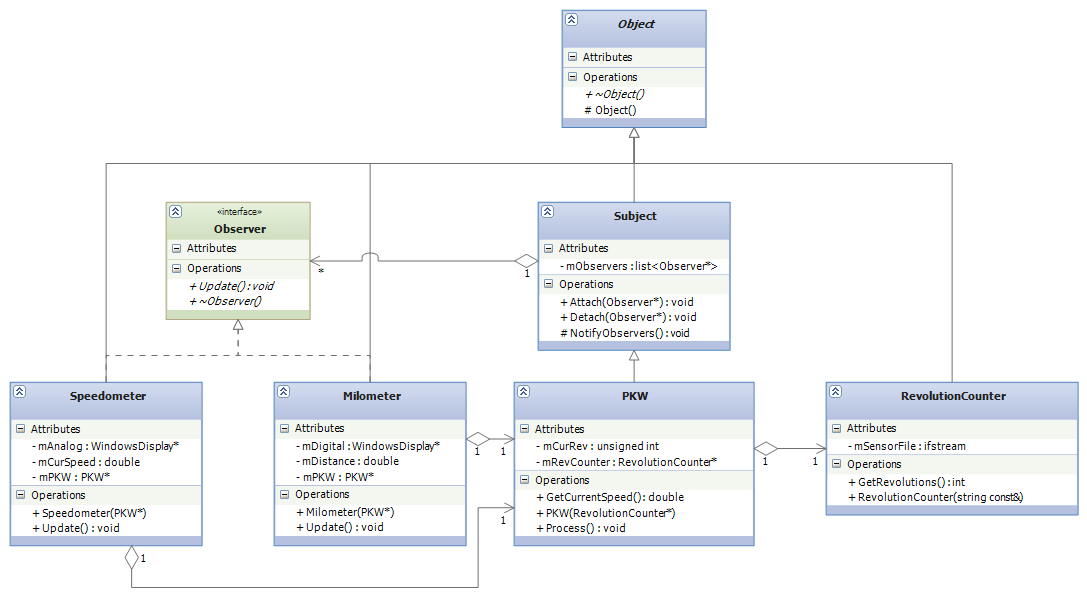
\includegraphics[angle=90,scale=0.85] {../Klassendiagramm.png}

\newpage
\subsection {Komponentenübersicht}
\begin {itemize} 
	\item Klasse "Object":
	\newline
	Basis aller Basisklassen.
	
	\item Klasse "Subject":
	\newline
	Basisklasse für Subjects, die überwacht werden.
	
	\item Interface "IObserver":
	\newline
	Interface für Observer.
	
	\item Klasse "Speedometer":
	\newline	
	Konkreter Observer, der die Momentangeschwindigkeit ermittelt. Überwacht PKW.
	
	\item Klasse "Milometer":
	\newline
	Konkreter Observer, der die gefahrenen Kilometer ermittelt. Überwacht PKW.
	
	\item Klasse "PKW":
	\newline
	Konkretes Subject, das überwacht wird.
	
	\item Klasse "RevolutionCounter":
	\newline
	Klasse die die Umdrehungen pro Minute zur Verfügung stellt.
		
\end {itemize}

\newpage
\section {Komponentenentwurf}
\subsection {Klasse "Object"}
Abstrakte Basisklasse aller Klassen. Von ihr werden alle anderen Klassen abgeleitet. Beinhaltet einen virtuellen Destruktor.

\subsection {Klasse "Subject"}
Hat eine Liste mit Zeigern auf Observer. Observer können via Methoden hinzugefügt, entfernt oder benachrichtigt.
\\

\textbf {Methode "Attach": } 
\newline
Schnittstelle: 
\newline
Parameter: Observer*
\newline
Rückgabetyp: void.
\newline
Fügt einen noch nicht vorhandenen Observer hinzu.
\\

\textbf {Methode "Detach": } 
\newline
Schnittstelle:
\newline
Parameter: Observer*
\newline
Rückgabetyp: void.
\newline
Entfernt einen Observer, wenn er vorhanden ist.
\\

\textbf {Methode "NotifyObservers": } 
\newline
Schnittstelle:
\newline
Rückgabetyp: void.
\newline
Ruft von allen Observern Update auf.
\\


\subsection {Interface "IObserver"}
Bietet die Schnittstelle für einen Observer. Hat einen virtuellen Destruktor.
\\

\textbf {Methode "Update": } 
\newline
Schnittstelle: 
\newline
Rückgabetyp: void.
\newline
Pure virtual function.
\\

\subsection {Klasse "Speedometer"}
Gibt die aktuelle Geschwindigkeit auf einem analogen Display aus.
\\

\textbf {Konstruktor "Speedometer": } 
\newline
Schnittstelle: 
\newline
Parameter: PKW*
\newline
Fügt den PKW hinzu und fügt dem PKW sich selbst zu. Fordert Speicher für ein neues Display an.
\\

\textbf {Methode "Update": } 
\newline
Schnittstelle: 
\newline
Rückgabetyp: void.
\newline
Ruft die Funktion GetCurrentSpeed von PKW auf und gibt den Wert dem analogen Display weiter.
\\

\subsection {Klasse "Milometer"}
Gibt die gefahrenen Kilometer auf einem Display aus.
\\

\textbf {Konstruktor "Milometer": } 
\newline
Schnittstelle: 
\newline
Parameter: PKW*
\newline
Fügt den PKW hinzu und fügt dem PKW sich selbst zu. Setzt die Kilometer auf 0. Fordert Speicher für ein neues Display an.
\\

\textbf {Methode "Update": } 
\newline
Schnittstelle: 
\newline
Rückgabetyp: void.
\newline
Ruft die Funktion GetCurrentSpeed von PKW auf, rechnet daraus die in den letzten 500ms gefahrenen Kilometer aus, addiert sie zu den gesamt gefahrenen Kilometern und gibt das Ergebnis dem analogen Display weiter.
\\


\subsection {Klasse "PKW"}
Stellt einen konkreten PKW dar. Hat einen Member, der die aktuellen Radumdrehungen speichert und einen der eine Referenz auf einen Radumdrehungszähler hat.
\\

\textbf {Konstruktor "PKW": } 
\newline
Schnittstelle:
\newline
Parameter: RevolutionCounter*
\newline
Fügt dem PKW einen Radumdrehungszähler hinzu.
\\

\textbf {Methode "GetCurrentSpeed": } 
\newline
Schnittstelle:
\newline
Rückgabetyp: double
\newline
Berechnet die aktuelle Geschwindigkeit.
\\

\textbf {Methode "Process": } 
\newline
Schnittstelle:
\newline
Rückgabetyp: void
\newline
Aktualisiert die aktuellen Radumdrehungen und benachrichtigt dann die Observer.
\\


\subsection {Klasse "RevolutionCounter"}
Klasse für die Radumdrehungen. Hat einen Member der den Filestream mit den Daten speichert. Im Konstruktor wird dieser Stream geöffnet, im Destruktor geschlossen.
\\

\textbf {Konstruktor "RevolutionCounter": } 
\newline
Schnittstelle:
\newline
Parameter: std::string const\& filename
\newline
Öffnet die gegebene Datei.
\\

\textbf {Methode "GetRevolutions": } 
\newline
Schnittstelle:
\newline
Rückgabetyp: int
\newline
Liest die Daten aus der Daten aus und gibt sie zurück.
\\

\newpage
\section {Source Code}

\lstinputlisting[language=C++]{\CodePath Object.h}
\lstinputlisting[language=C++]{\CodePath Object.cpp}
\newpage

\lstinputlisting[language=C++]{\CodePath Subject.h}
\newpage
\lstinputlisting[language=C++]{\CodePath Subject.cpp}
\newpage

\lstinputlisting[language=C++]{\CodePath IObserver.h}
\newpage

\lstinputlisting[language=C++]{\CodePath Milometer.h}
\newpage
\lstinputlisting[language=C++]{\CodePath Milometer.cpp}
\newpage

\lstinputlisting[language=C++]{\CodePath Speedometer.h}
\newpage
\lstinputlisting[language=C++]{\CodePath Speedometer.cpp}
\newpage

\lstinputlisting[language=C++]{\CodePath PKW.h}
\newpage
\lstinputlisting[language=C++]{\CodePath PKW.cpp}
\newpage

\lstinputlisting[language=C++]{\CodePath RevolutionCounter.h}
\newpage
\lstinputlisting[language=C++]{\CodePath RevolutionCounter.cpp}
\newpage

\lstinputlisting[language=C++]{\CodePath Main.cpp}
\newpage

\section {Testausgaben} 

\begin {verbatim}
Testcase0: File does not exist.
RevolutionCounter.cpp::RevolutionCounter: error in open file
Process RevEntries: ... RevolutionCounter.cpp::GetRevolutions: 
end of data
Done


Testcase1: Empty file without fill function.
Process RevEntries: ... Done


Testcase2: Empty file with fill function.
Process RevEntries: ... Done


Testcase3: File with invalid content.
Process RevEntries: ... RevolutionCounter.cpp::GetRevolutions: 
conversion string to int failed
RevolutionCounter.cpp::GetRevolutions: conversion string to int failed
RevolutionCounter.cpp::GetRevolutions: conversion string to int failed
RevolutionCounter.cpp::GetRevolutions: conversion string to int failed
RevolutionCounter.cpp::GetRevolutions: conversion string to int failed
RevolutionCounter.cpp::GetRevolutions: conversion string to int failed
RevolutionCounter.cpp::GetRevolutions: conversion string to int failed
Done


Testcase4: File with a single entry.
Process RevEntries: ... Done


Testcase5: File with a single entry and too much Process calls.
WindowsClient: Server not online. Waiting...
WindowsClient: Server not online. Waiting...
WindowsClient: Server not online. Waiting...
WindowsClient: Server not online. Waiting...
Process RevEntries: ... RevolutionCounter.cpp::GetRevolutions: 
end of data
RevolutionCounter.cpp::GetRevolutions: end of data
Done


Testcase6: File with multiple entries.
Process RevEntries: ... Done
\end {verbatim}


\end{document}